\documentclass[11pt, oneside]{article} 
\usepackage{geometry}
\geometry{letterpaper} 
\usepackage{graphicx}
	
\usepackage{amssymb}
\usepackage{amsmath}
\usepackage{parskip}
\usepackage{color}
\usepackage{hyperref}

\graphicspath{{/Users/telliott/Github/figures/}}

\title{Similar triangles}
\date{}

\begin{document}
\maketitle
\Large

%[my-super-duper-separator]

To repeat what we said before, some triangles may be \emph{similar} but not congruent.

Similarity means that the three angles are the same but the triangles are of different overall sizes.  We might say that they are the same but \emph{scaled} differently.

We can call this AAA (angle-angle-angle).

\begin{center} 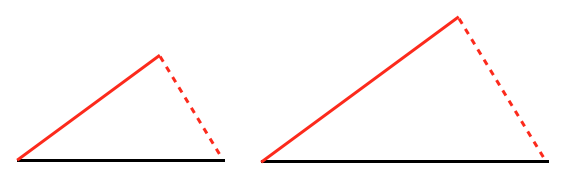
\includegraphics [scale=0.4] {similar.png} \end{center}

Actually, there are three statements which are equivalent, but need to be proved equivalent as theorems.  This isn't always done carefully.

$\bullet$  Two triangles are similar if they have the same three angles. 

$\bullet$  Two triangles are similar if their sides are parallel to one another. 

$\bullet$  Two triangles are similar if their sides are in the same ratio to each one another. 

Because of the angle sum theorem, if any two angles of a pair of triangles are known to be equal, then the third one must be equal as well.

$\bullet$  Two triangles are similar if they have two angles known to be equal. 

For similar triangles, the three corresponding pairs of sides are in the same proportions, but re-scaled by a constant of proportion.  This is known as the AAA similarity theorem.

Before getting there we introduce another theorem.

\subsection*{midline theorem}

Theorem:  The line segment $BC$ connecting the midpoints of two sides of a triangle is parallel to the third side, and is congruent to half of it.

\begin{center} 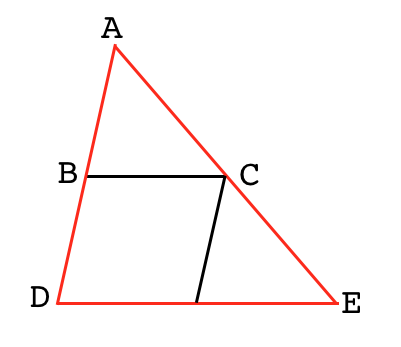
\includegraphics [scale=0.4] {similar11.png} \end{center}

Earlier we said that in a triangle like the one in the figure below, if we are given that $BC$ is parallel to $DE$, then by the a combination of the alternate interior angles theorem and the vertical angles theorem, we can show that $\triangle ABC$ and $\triangle ADE$ have three angles the same.

\begin{center} 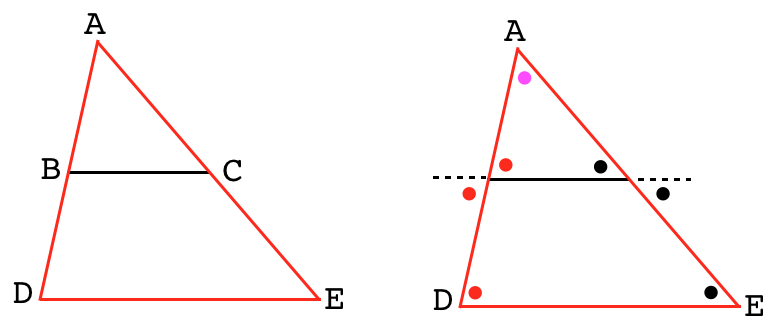
\includegraphics [scale=0.4] {similar6.png} \end{center}

Their sides are also in proportion.  How can we prove that?  

Let us start with the case where $AB = BD$.  Draw similar line segments parallel to $AE$ and parallel to $AD$.

\begin{center} 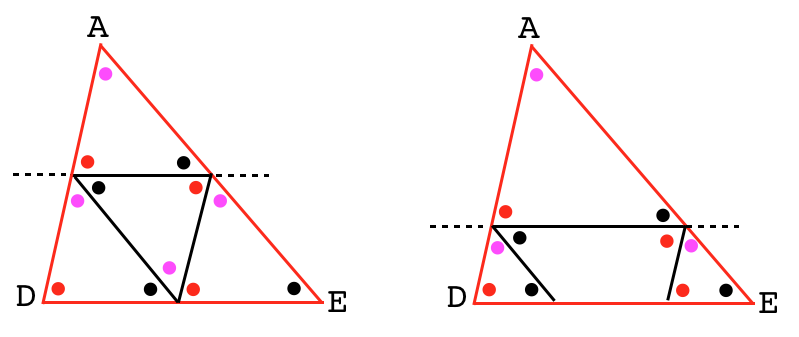
\includegraphics [scale=0.4] {similar9.png} \end{center}

Notice that something nice happens on the left, in the case where $AB = BD$.  To see why, it may be useful to take a side track and look at parallelograms, which are basically triangles that have been stitched together.

\begin{center} 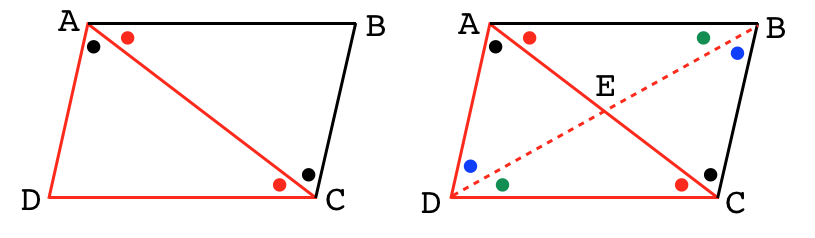
\includegraphics [scale=0.4] {pgram1.png} \end{center}

The definition of a parallelogram is that it is a four-sided figure with opposing sides parallel.  Thus, the interior angles theorem gives us the angle equalities shown.  On the left, we have three angles the same and a shared side, hence $\triangle ABC \cong \triangle ACD$.  We have shown that $AB = DC$ and $AD = BC$.

If we draw the other diagonal and change nothing else, opposing triangles are congruent by ASA.  Therefore, the diagonals cross at their midpoints.

If we further constrain all the sides to be equal, then the half triangles like $\triangle ADC$ become isosceles.  

The isosceles triangle theorem says that in a triangle with two sides equal the base angles are equal.  The converse is also true.  Note that in the proof of the isosceles triangle theorem, we do not use any facts about similar triangles, only congruent ones!

By the isosceles triangle theorem, all the angles marked with red dots are equal, and all the blue ones as well.  Because each quarter triangle has a red and a blue, the central angles are all equal.  Therefore, they are all right angles.

\begin{center} 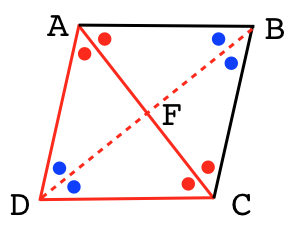
\includegraphics [scale=0.4] {pgram2.png} \end{center}

Now, finally, let us assemble one whole and two half parallelograms starting with the same figure.

\begin{center} 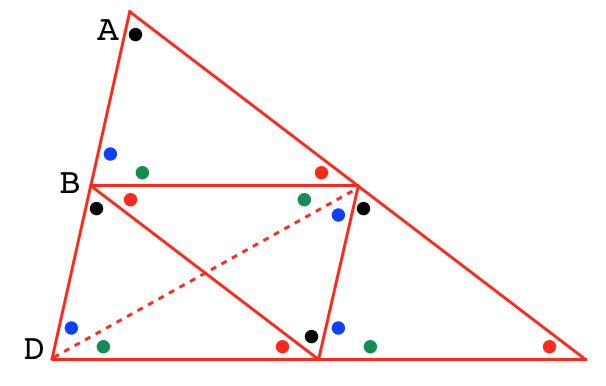
\includegraphics [scale=0.4] {pgram4.png} \end{center}

By the properties of the parallelogram, if the adjacent sides $AB$ and $BD$ are equal, all the angles work out and we get four congruent triangles, so the adjacent sides of the large triangle all have equal segments as well.

So finally, what about the case where the adjacent segments are not equal?  Good question!

\subsection*{AAA similarity theorem}

The proof comes in two parts, first for the angles, and then for the ratio of sides.

The main theorem used for angle identity is the alternate interior angles theorem, which is an if and only if theorem:  such angles are equal $\iff$ there is a transversal of two parallel lines.

\begin{center} 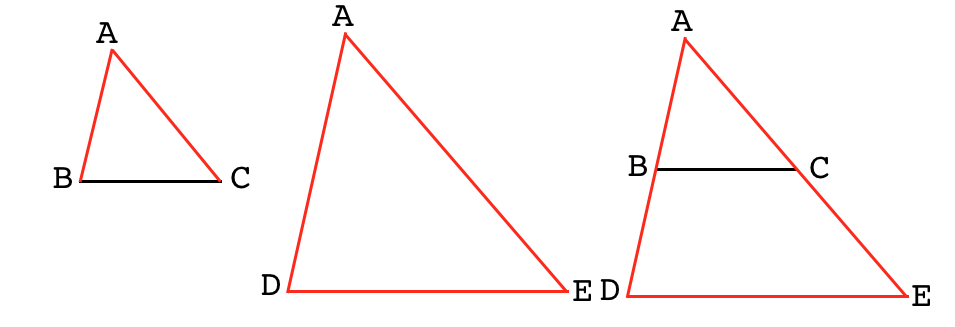
\includegraphics [scale=0.4] {similar10.png} \end{center}

Suppose we have $\triangle ABC$ and separately $\triangle ADE$ and we are given that the angle at vertex $A$ is the same for both, and when we draw $\triangle ABC$ on top of $\triangle ADE$, $BC$ is parallel to $DE$.

By the alternate interior angles theorem, $\angle ABC =  \angle ADE$ and  $\angle ACB = \angle AED$.

\begin{center} 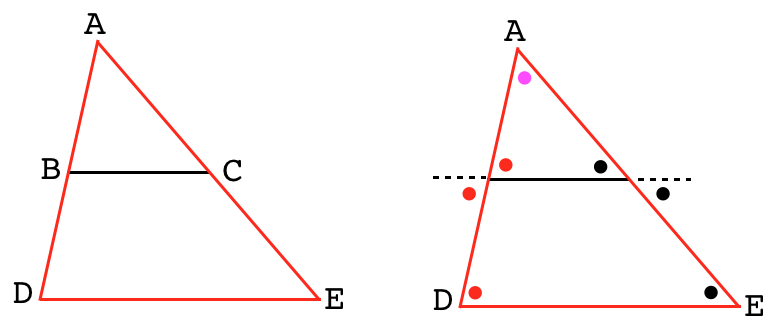
\includegraphics [scale=0.4] {similar6.png} \end{center}

Proving that the ratios of sides are all the same is a bit harder and often not even done explicitly.  I found a good proof in Kiselev.

\begin{center} 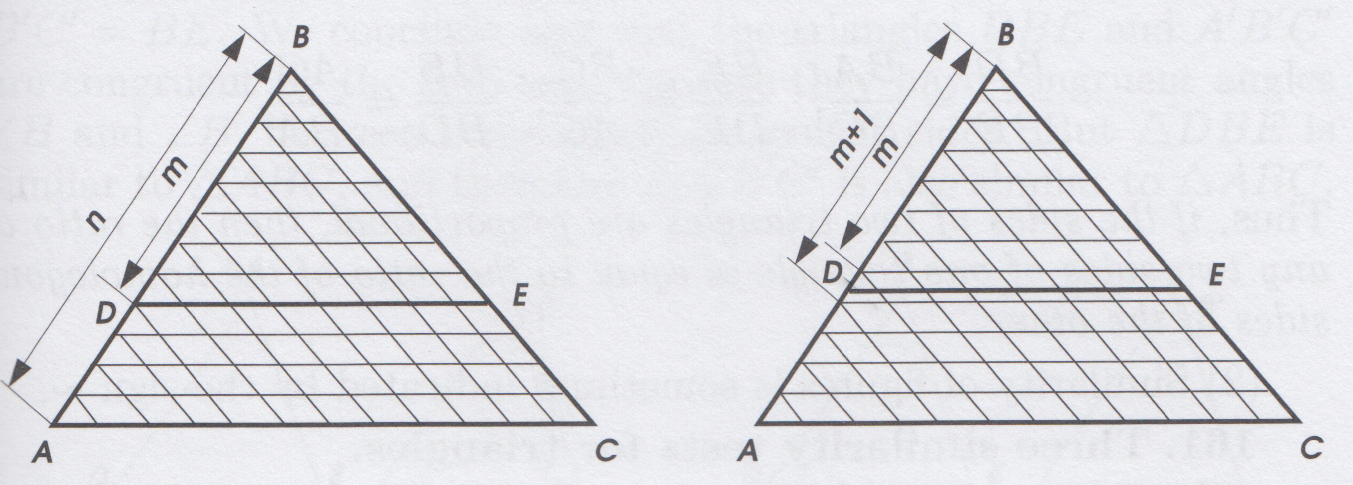
\includegraphics [scale=0.25] {Kiselev166.png} \end{center}

(Note:  he draws $\triangle BDE$ smaller than $\triangle BAC$).

There are two cases.  The first is when the lengths of $BA$ and $BD$ are commensurable.  That is, there is some unit length such that for integers $m$ and $n$, $BD = m$ and $BA = n$.

Divide the side as shown.  Draw lines parallel to $BC$ and $AC$.  

Then $BE$ and $BC$ will be divided into congruent parts, $m$ and $n$ for each, respectively.  The same thing happens on the bottom.  It is clear that 
\[ \frac{m}{n} = \frac{BD}{BA} = \frac{DE}{AC} = \frac{BE}{BC} \]

The second case is shown in the right panel above.  $BD$ and $BA$ are not commensurate and there is some small remainder when dividing $m$ into $n$.  But 
\[ \frac{m}{n} \approx \frac{BD}{BA}, \ \ \ \ \ \ \frac{m}{n} \approx \frac{DE}{AC}, \ \ \ \ \ \ \frac{m}{n} \approx  \frac{BE}{BC} \]

And furthermore, by choosing $n$ larger, we can make the remainder as small as we please.  Thus we obtain, in the limit and $n$ gets very large:
\[ \frac{m}{n} = \frac{BD}{BA} = \frac{DE}{AC} = \frac{BE}{BC} \]
for the second case as well.

\subsection*{another idea}

Euclid doesn't get around to proving the AAA similarity theorem until Book VI.

If you look at the chapter on the Pythagorean theorem, you will see that Euclid's proof from $PI.47$ depends only on triangle congruence and not anything about similarity.  Therefore, we can rely on it here.

Here is a sketch for a proof.

We also have an algebraic proof of Pythagoras which starts from this figure:
\begin{center} 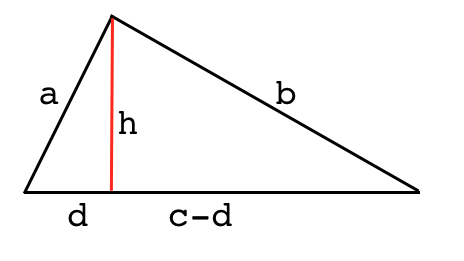
\includegraphics [scale=0.45] {pythagoras5.png} \end{center}

and assumes the side ratios of similar right triangles 

hypotenuse to short side
\[ \frac{a}{d} = \frac{b}{h} = \frac{c}{a} \]
hypotenuse to long side
\[ \frac{a}{h} = \frac{b}{c-d} = \frac{c}{b} \]

and so goes on to prove the Pythagorean theorem.  You can run this proof backwards from the theorem to the side ratios result.  Therefore, AAA similarity is established for right triangles.

Then, any triangle can be decomposed into two right triangles.  So, combining the results for the two sub-triangles, we would have the result for the general case.

Here is a sketch of that part:

\begin{center} 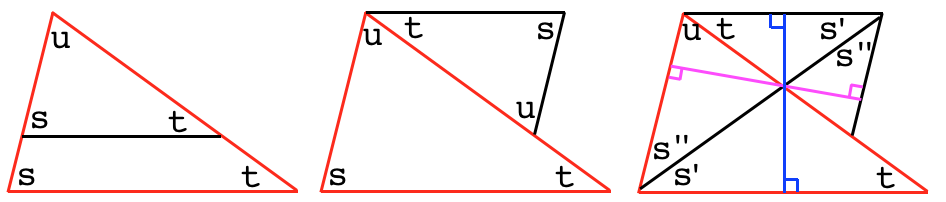
\includegraphics [scale=0.45] {similar12.png} \end{center}

We have two triangles similar because the angles are the same (left panel).  Flip the smaller triangle up and form a partial parallelogram.  The original small triangle and the flipped version are congruent by SAS.

From the parallel sides we get the angle equalities in the right panel.  Draw the two altitudes.

Now we have various similar right triangles.  Composing the results for the right triangles, we can build up to the main result.

\subsection*{pyramid height}
As we said, Thales was from Miletus and he lived around 600 BC.  Thales is believed to have traveled extensively and was likely of Phoenician heritage.  As you probably know, the Phoenicians were famous sailors who founded many settlements around the Mediterranean.  

They competed with the mainland Greeks and later with the Romans for colonies, and their major city, Carthage, was destroyed much later by the Romans in the third Punic War.  

During his travels, Thales went to Egypt, home to the great pyramids at Giza, which were already ancient then.  They had been built just around around 2560 BC (dated by reference to Egyptian kings) and were already 2000 years old at that time!

The story is that Thales asked the Egyptian priests about the height of the Great Pyramid of Cheops, and they would not tell him.  So he set about measuring it himself.  The current height is 480 feet.  He used similar triangles.

\begin{center} 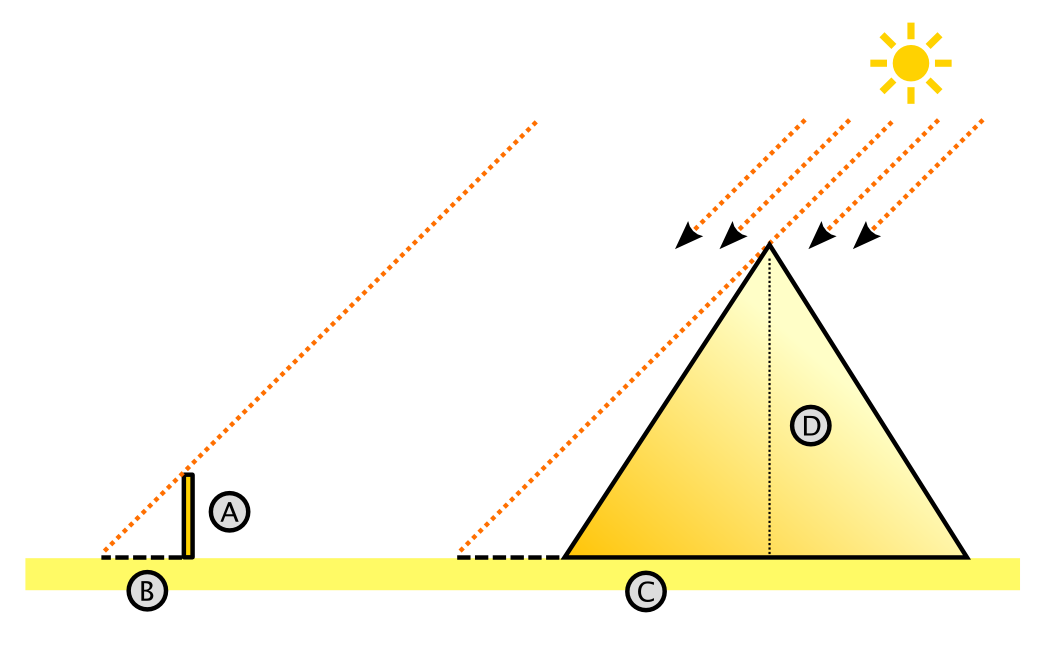
\includegraphics [scale=0.25] {Thales_theorem_6.png} \end{center}

\end{document}